% DO NOT COMPILE THIS FILE DIRECTLY!
% This is included by the other .tex files.

\begin{frame}[t,plain]
\titlepage
\end{frame}


\begin{frame}
\frametitle{MISP - Open Source Threat Intelligence Platform}
        \begin{itemize}
                \item MISP is an open source software (can be self-hosted or cloud-based) {\bf information sharing and exchange platform}
                \item It enables analysts from different sectors/orgs to create, collaborate on and share information
                \item The information shared can then be used to find correlations as well as automatically be fed into {\bf protective tools or processes}
                \item The software is widely used by CERTs, ISACs, Intelligence Community, military organisations, private sector organisations and researchers since 2012
                \item CIRCL is both the main driving force behind the tool's {\bf development} as well as some of the largest information {\bf sharing communities} worldwide
        \end{itemize}
\end{frame}

\begin{frame}
        \frametitle{MISP Project Overview}
        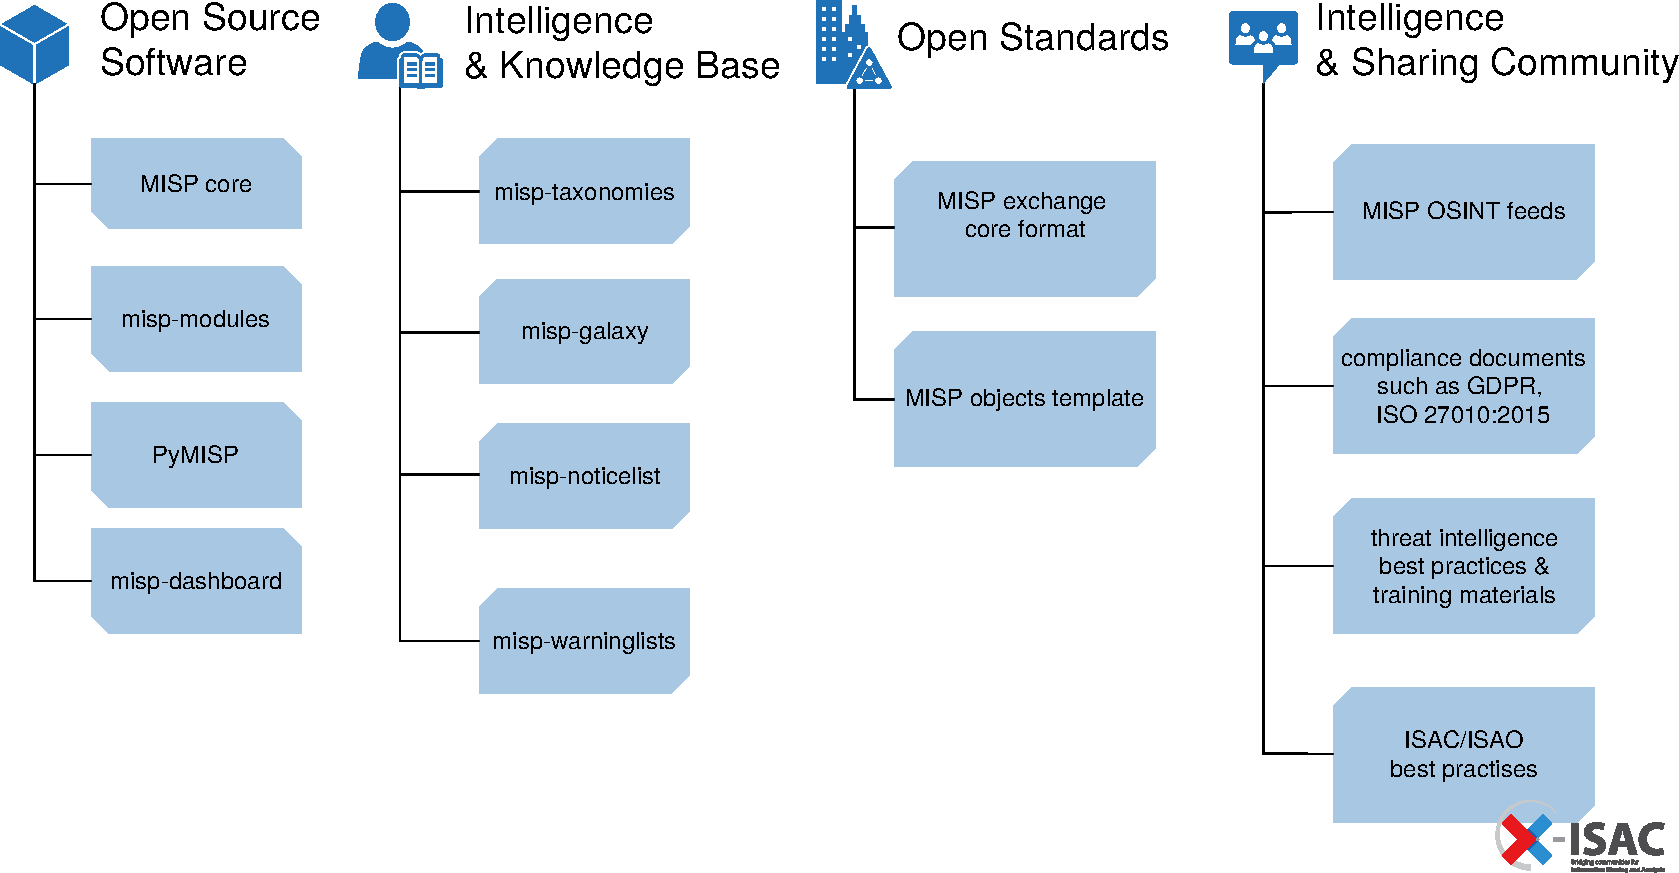
\includegraphics[scale=0.42]{misp-overview-simplified.pdf}\\
\end{frame}


\begin{frame}
\frametitle{MISP core distributed sharing functionality}
\begin{itemize}
\item MISP's core functionality is sharing where everyone can be a consumer and/or a contributor/producer.
\item Quick benefit without the obligation to contribute.
\item Low barrier access to get acquainted to the system.
\end{itemize}
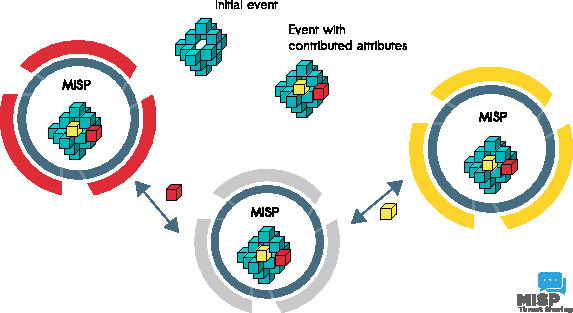
\includegraphics[scale=0.9]{misp-distributed.pdf}
\end{frame}

\begin{frame}
\frametitle{DFIR and MISP digital evidences}
        \begin{itemize}
                \item {\bf Share analysis and report} of digital forensic evidences.
                \item {\bf Propose changes} to existing analysis or report.
                \item Extending existing event with additional evidences for local or limited use (sharing can be defined at event level or attribute level).
                \item {\bf Evaluate correlations}\footnote{MISP has a flexible correlation engine which can correlate on 1-to-1 value but also fuzzy hashing (e.g. ssdeep) or CIDR block matching.} of evidences against external or existing attributes.
                \item {\bf Report sighting} such as false-positive or true-positive (e.g. a partner/analyst has seen a similar indicator).
        \end{itemize}
\end{frame}

\begin{frame}
\frametitle{Benefits of using MISP}
\begin{itemize}
        \item  LE can leverage the long-standing experience in information sharing and {\bf bridge their use-cases} with MISP's information sharing mechanisms.
        \item {\bf Accessing existing MISP information sharing communities} by getting actionable information from CSIRTs/CERTs networks or security researchers.
        \item {\bf Bridging LE communities with other communities}. Sharing groups can be created (and managed) between cross-sectors to support specific use-cases.
        \item {\bf MISP standard format} is a flexible format which can be extended by the users who use the MISP platform. A MISP object template can be created in 30 minutes and directly share information with your model towards existing communities.
\end{itemize}
\end{frame}

\begin{frame}
        \frametitle{Future of Information Sharing}
        \begin{itemize}
        \item MISP is a long-term project (started in 2012) and since {\bf information sharing is becoming more essential} than ever to thwart threats, we have long-term plans for the project as the project is used in various critical information exchange communities.
        \item We hope to have the means to be the enablers and the interface for real cross-sectorial sharing and support the organisations facing hybrid threats.
        \item Tools, open standards and interoperable software (e.g. DFIR tools) are driving forces behind resilient information exchange communities.
        \item Getting ideas and practical {\bf use-cases from LE community} is vital, don't hesitate to interact.
        \end{itemize}
\end{frame}


